\chapter{Criptografía de clave pública}
\section{De la criptografía clásica a la de clave pública}
%TODO. Comentar algo de la historia que propició este cambio. Está en las transparencias.

\subsection{Enigma}
La máquina \textbf{enigma} funcionaba de acuerdo al siguiente esquema:
\begin{center}
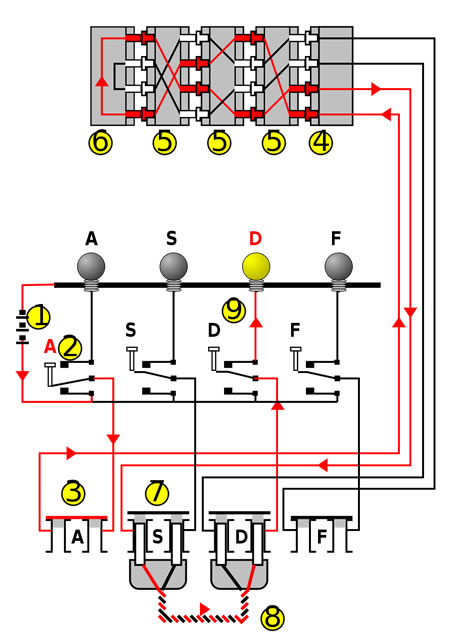
\includegraphics[width=0.6\textwidth]{img/enigma.jpg}
\end{center}
donde el número 8 representa uno de los modificadores, que simplemente conectaba pares de letras para que fuesen intercambiadas; el número 5 representa los rotores y el número 6 el reflector.

En rojo podemos ver el flujo que seguiría la corriente en caso de que pulsásemos la letra $A$, que sería cifrada a una $D$.

\obs La configuración que se muestra en la imagen sólo se mantendría fija durante un brevísimo periodo de tiempo. Tras finalizar el cifrado de la letra $A$, los rotores girarían de modo que no se volvería a seguir el mismo camino nunca más.

Si tenemos una máquina de enigma que funcione con 26 letras, 5 rotores de entre los que hay que escoger 3 y modificando 6 pares de letras\footnote{Es decir, tenemos 6 modificadores}, la pregunta que surge es clara, ¿Cuántas claves posibles tenemos?

Para empezar tenemos que escoger qué tres rotores tomamos, teniendo en cuenta que importa el orden, con lo que tenemos $5\cdot 4 \cdot 3 = 60$ opciones posibles.

Una vez hemos escogido los rotores, debemos ver qué posición tendrá cada rotor. Puesto que tenemos 26 posiciones para cada rotor tenemos un total de $26^3$ opciones.

Por último debemos colocar los modificadores, para lo que tenemos que elegir 6 pares de letras. Para ello tenemos un total de
\[{26 \choose 2} \cdot {24\choose 2}\cdot {22\choose 2}\cdot {20\choose 2}\cdot {18\choose 2}\cdot {16\choose 2} \text{ opciones }\]

Pero, puesto que no importa el orden, debemos dividir entre $6!$.

Agrupando todo lo que hemos mencionado, tenemos que la máquina \textbf{enigma} permite tener un total de:
\[\frac{60\cdot 26^3 \cdot {26 \choose 2} \cdot {24\choose 2}\cdot {22\choose 2}\cdot {20\choose 2}\cdot {18\choose 2}\cdot {16\choose 2}}{6!}\approx 8.469 \cdot 10^{17}  \text{ claves }\]

La forma de trabajar con \textbf{enigma} era mediante un libro de claves donde cada clave era empleada a lo largo de todo el día para todas las comunicaciones.

No obstante, si toda la flota empleaba el mismo sistema de cifrado y los mensajes eran fácilmente interceptables (se comunicaban por radio) al final sería relativamente sencillo que el enemigo descifrara la clave. Para solucionar esto, lo que se hacía es que al comienzo de cada mensaje se enviaban 3 letras, que indicaban la nueva posición de los rotores que debería emplearse a partir de ese momento.

Así, un esquema de transmisión del mensaje sería:
\begin{enumerate}
\item Montamos la máquina con la clave del día.
\item Transmitimos la clave del mensaje dos veces.
\item Cambiamos la posición de los rotores según la clave que enviamos.
\item Transmitimos el mensaje.
\end{enumerate}

Aquí tenemos la debilidad del criptosistema, el envío de la clave dos veces, puesto que nos adelanta cierta información acerca de la posición inicial de los rotores. Otro problema radicó en el hecho de que el primer mensaje del día siempre informaba del tiempo y siempre comenzaba de la misma forma, lo que daba aún más información a los enemigos.

A la hora de descifrar, el mecanismo es sencillo. La forma en que funciona \textbf{enigma} está basada en trasposiciones. Es decir, si a partir de la letra $A$ obtengo la $B$, a partir de la $B$ obtendré la $A$, partiendo de la misma clave.

Por tanto, una vez recibido el mensaje lo único que hay que hacer es introducir el mensaje cifrado en la máquina y como salida obtendremos el texto original.

Veamos por qué estos es cierto:
\begin{proof}
Para comprobar que la función de cifrado y su inversa son la misma, vamos a ver cómo funcionaba \textbf{enigma} sobre cada letra.

En primer lugar se intercambiaba una letra por otra mediante los modificadores. Tras esto la letra pasa por los rotores y llega al reflector (que será la clave de la demostración) y tras ello vuelve a pasar por los rotores y por el modificador.

Así nos queda que
\[\rho(m) = σ^{-1}δ^{1}Rδσ(m) \implies \rho^{-1}(m) = σ^{-1}δ^{1}Rδσ(m) = \rho(m)\]
\end{proof}

Pero ahora el lector avispado se percatará de un detalle muy importante. De todas las claves posibles que mencionamos al inicio de esta sección, no todas darán lugar a una función $\rho$ que coincida con su inversa.

En este caso, $\rho = \rho^{-1} \iff \rho = (a_1a_2)(a_3a_4)...(a_{25}a_{26})$, puesto que necesitamos que $\rho$ no haga más que permutar pares de letras.

Dada esta restricción tendremos un total de
\[\frac{{26 \choose 2} {24 \choose 2} ... {2 \choose 2}}{13!} =\frac{26!}{13!2^{13}} \approx 1.01 \cdot 10^{15} \text{ claves posibles }\]

\subsection{Criptosistemas de clave simétrica}
Todos los sistemas que hemos visto hasta ahora, englobados como criptosistemas clásicos, comparten una misma propiedad: \textit{Si sabemos cómo cifrar sabremos cómo descifrar}. Esto se debe a que todos estos sistemas son de \textbf{clave simétrica}.

Si pretendemos que diferentes usuarios puedan emplear el mismo criptosistema manteniendo seguridad entre ellos, neceistaremos una clave distinta para cada uno de ellos.

En el mundo de la tecnología en que vivimos ahora mismo esto es inviable puesto que serían necesarias demasiadas claves (una por usuario/actividad). Además, al llegar un nuevo usuario sería necesario compartir con él la clave de alguna forma.

La solución es la función $3^{n}$ en $\mathbb{F}_{1231}^*$:
% TODO imagen de la función

\begin{defn}[Función de un sólo sentido]
Sea $\appl{f}{A}{B}$ una función inyectiva, se dice que es \textbf{de un sólo sentido} si:
\begin{enumerate}
\item $f(a)$ es fácil de calcular
\item Dado $b \in Im(f)$ podemos encontrar $a\tq f(a) = b$ pero, en la práctica, es difícil de encontrar.
\end{enumerate}
\end{defn}

Como ejemplo trivial podemos considerar un puzle y la función $f$ que consiste en desmontarlo. Esta función es trivial, basta con darle una patada al puzle, pero su inversa, que sería montar el puzle de nuevo, es compleja de calcular.

Vamos a definir formalmente dos adjetivos que emplearemos al referirnos a diferentes problemas:

\begin{defn}[Fácil]
Si $k$ es el tamaño de los datos, el tiempo necesario para resolver el problema es polinómico en $k$, es decir $T=O(k)$
\end{defn}

\begin{defn}[Difícil]
Si $k$ es el tamaño de los datos, el tiempo necesario para resolver el problmea es no polinómico. Puede ser exponencial $T=O(e^k)$, o subexponencial $T=e^{\sqrt{k}}$ entre otros
\end{defn}

\subsection{Estimaciones de tiempo}

Los datos con los que vamos a trabajar serán, de un modo u otro, números. Por tanto debemos ser capaces de estimar cómo son estos números, a fin de ver si son manejables o no.

El tamaño de $n \in \ent$ puede venir dado por $\log(n)$. Nos da igual el tipo de logaritmo que escojamos puesto que la relación entre logaritmos viene dada por una constante.

Vamos a definir ahora una medida de unidad del tiempo.

\begin{defn}[Bit-operación]
Denominamos \textbf{bit-operación} al proceso de sumar dos bits.
\end{defn}

\begin{example}
¿Cuánto tiempo es necesario para sumar dos enteros de $k$ y $l$ bits respectivamente?

Sin pérdida de generalidad podemos suponer que $k\geq l$. En ese caso tendremos que hacer un total de $k$ bit-operaciones.

En general, si estamos trabajando con números menores que $N$ (como ocurre al movernos en $\ent_N$), el tiempo empleado será $T= O (\log(N))$
\end{example}

\begin{example}
¿Cuánto tiempo empleamos para multiplicar dos números enteros de $k$ y $l$ bits respectivamente?

Recordando el procedimiento realizado para multiplicar números cuando estábamos en el colegio podemos ver que tendremos que realizar un total de $l-1$ sumas de $l+k-1$ dígitos.

Así, considerando $k \geq l$, el tiempo que necesitaremos será de la forma $(l-1)O(k+l-1) = O(k)O(k)=O(k^2)$

\end{example}

En este último ejemplo podemos encontrar diferentes excepciones en función de la forma en que se realice la multiplicación. Por ejemplo, si multiplicamos empleando la transformación de Fourier rápida tendríamos $T=O(\log(N) \log(\log(N)) = O(k \log ( k ))$.

Estos ejemplos (a los que podemos añadir el caso de la división) consistuyen ejemplos de operaciones que pueden realizarse en tiempo polinómico, es decir, serían catalogados como problemas fáciles.

Veamos otro ejemplo un poco más interesante:

\begin{example}
¿Cuánto tiempo es necesario para calcular la exponencial módulo N?

Lo que haremos para calcular esta exponencial será multiplicar la base por sí misma una vez tras otra, realizando el cálculo del módulo cuando sea necesario. Es decir, en cada paso tendremos $T=O(k^2)+O(k^2) = O(k^2)$, es decir, la suma de los tiempos empleados en la multiplicación y la correspondiente división.

Además, esta operación se llevará a cabo un máximo de $N$ veces, (puesto que no tiene sentido poner un exponente mayor). Por tanto, el tiempo total será $T=O(\log^2(N))\cdot O(N) = O(N\log^2(N))$

No obstante, hasta aquí estamos considerando que estamos multplicando de la forma más lenta posible. Es decir, estamos calculando $3^x = (((3\cdot 3)\cdot 3) \cdot 3) ...$.

Si agrupamos los factores obtenidos al descomponer la potencia en productos de dos en dos, tendremos que el número de productos necesarios será mucho menor.

En general, empleando el algoritmo de los cuadrados iterados requiere un tiempo total de $O(\log^2(N))$.
\end{example}

\begin{example}
¿Cuánto tiempo es necesario para realizar un cambio de base?

El razonamiento del resultado queda como ejercicio para el lector.

El tiempo empleado será $T=O(k^3)$.

Conocido este resultado, podemos ver que para calcular la exponencial, aunque tengamos que realizar un cambio de base para movernos cómodamente en base 2, tendremos un tiempo total $T=O(k^3)+O(k^4)=O(k^4)$, es decir, \textbf{exponenciar} es un proceso fácil.

\end{example}

\begin{defn}[Problema del logaritmo discreto]
Sea $G=<g>$ un grupo cíclico de orden $N$, es decir, $G=\{g^i \}$, el \textbf{problema del logaritmo discreto, DLP} para $G$ consiste en encontrar $i \tq h=g^i$ dado $h \in G$.

El mejor algoritmo conocido para resolver el $DLP$ en $(\ent_p)^*$ necesita tiempo subexponencial.
\end{defn}

\begin{corol}
El problema $DLP$ con $\appl{f}{(\ent_p)^*}{(\ent_N) *}$ es de un dólo sentido si $p$ es suficientemente grande.
\end{corol}